
\documentclass[tikz]{standalone}
\usepackage{tikz}
\usetikzlibrary{fit}
\usepackage[dvipsnames]{xcolor}
\usetikzlibrary{positioning, arrows.meta, calc, decorations.pathreplacing}
\definecolor{lightblue}{RGB}{173, 216, 230}
\begin{document}
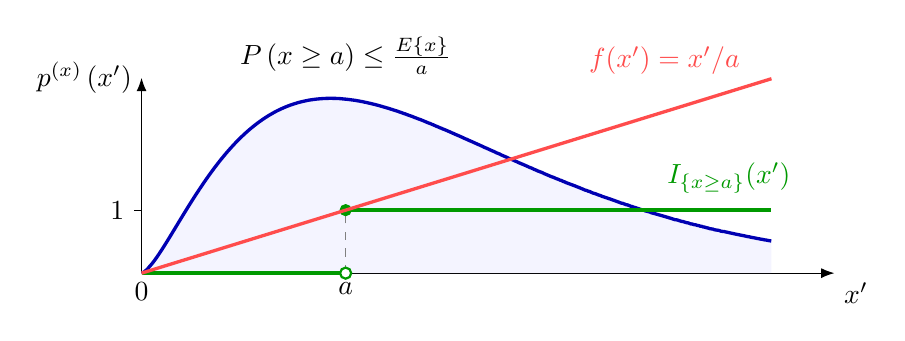
\begin{tikzpicture}[scale=1, x=0.8cm, y=0.8cm]
 \def\a{3.24}
 \def\xmax{10}
 \def\m{0.02}
 \draw[-{Latex}] (0,0) -- (\xmax+1,0) node[below right] {$x'$};
 \draw[-{Latex}] (0,0) -- (0,3.1) node[left] {$p^{(x)}\left(x'\right)$};
 \fill[blue!15, opacity=0.3]
 plot[samples=400, domain=0:\xmax, smooth]
 (\x,{ (6/sqrt(2*pi)) * (\x)^(1.5) * exp(-\x/2) }) -- (\xmax,0) -- (0,0) -- cycle;
 \draw[blue!70!black, very thick, samples=400, domain=0:\xmax, smooth]
 plot (\x,{ (6/(sqrt(2*pi))) * (\x)^(1.5) * exp(-\x/2) })
 node[pos=0.9, above right, xshift=2pt] {};
 \draw[dashed, gray] (\a,0) -- (\a,1.05);
 \node[below] at (\a,0) {$a$};
 \node[above] at (1*\a,3) {$\mathbb{P}\left(x \geq a\right) \leq \frac{\mathbb{E} \{ x\}}{a}$};
 \node[below] at (0,0) {$0$};
 \draw[green!60!black, ultra thick] (0,0) -- (\a,0);
 \filldraw[white, draw=green!60!black, line width=0.8pt] (\a,0) circle (2pt);
 \draw[green!60!black, ultra thick] (\a,1) -- (\xmax,1)
 node[pos=0.9, above, yshift=2pt] {$\mathbb{I}_{\{x \ge a\}}(x')$};
 \filldraw[green!60!black] (\a,1) circle (2pt);
 \draw[red!70, very thick, samples=2, domain=0:\xmax]
 plot (\x,{ \x*(1/\a) });
 \node[align=right,red!70,yshift=20pt] at ({2.5*\a+0.2},{2.5}) {$f(x') = x'/a$};
 \draw (0,1) -- ++(-0.12,0) node[left] {$1$};
 \end{tikzpicture}
\end{document}
